% IngredientIQ research paper: CONDENSED 10-PAGE VERSION of main.tex.
% Same findings, numbers, figures and references as main.tex; shorter prose, compact (pivoted) tables,
% tighter layout. Build exactly like main.tex (Overleaf, pdfLaTeX; or latexmk -pdf main_10page.tex).
% Compact tables (tables/*_compact.tex) are generated by scripts/make_paper_assets.py: never edit by hand.
% House style: no em dashes anywhere (use commas, colons, semicolons or parentheses).
%
% What changed versus main.tex, to fit 10 pages:
%   - margins 2.5cm -> 2cm; tighter paragraph, heading, list, float and table spacing
%   - Objectives as one paragraph; Literature Survey subsections 2.1-2.4 merged into one discussion
%   - Table 2 (dataset construction) folded into the text of Section 3.1
%   - Tables 4-8 pivoted to one row per scope and target (tables/*_compact.tex)
%   - Fig. 6 (ablation scores) dropped: its numbers are in the ablation table
%   - Table 8 (sensitivity) summarised in the text; tables/tab_sensitivity_compact.tex is ready
%     to \input if a page is to spare
\documentclass[11pt,a4paper]{article}
\usepackage[a4paper,margin=2cm]{geometry}
\usepackage[T1]{fontenc}
\usepackage[sfdefault]{carlito}          % metric clone of Calibri, as in the template
\usepackage{amsmath,amssymb}
\usepackage{graphicx}
\usepackage[table]{xcolor}
\usepackage{array,longtable,tabularx}
\usepackage{xspace}
\usepackage{enumitem}
\usepackage{titlesec}
\usepackage[labelsep=colon,font={small,it},skip=4pt]{caption}
\usepackage{tikz}
\usetikzlibrary{arrows.meta,positioning}
\usepackage[colorlinks=true,urlcolor=linkblue,linkcolor=black,citecolor=black]{hyperref}
\usepackage{xurl}
\graphicspath{{figures/}}

\definecolor{headblue}{RGB}{46,116,181}   % heading colour of the template
\definecolor{headfill}{RGB}{217,226,243}  % table header shading
\definecolor{groupfill}{RGB}{242,242,242} % table group rows (e.g. "All, Rating")
\definecolor{linkblue}{RGB}{5,99,193}

% Floats share pages with text; less white space around them
\renewcommand{\topfraction}{0.92}
\renewcommand{\bottomfraction}{0.8}
\renewcommand{\textfraction}{0.06}
\renewcommand{\floatpagefraction}{0.88}
\setcounter{topnumber}{3}
\setcounter{totalnumber}{4}
\setlength{\textfloatsep}{8pt plus 2pt minus 2pt}
\setlength{\floatsep}{8pt plus 2pt minus 2pt}
\setlength{\intextsep}{8pt plus 2pt minus 2pt}

\titleformat{\section}{\color{headblue}\Large\bfseries}{\thesection.}{0.4em}{}
\titleformat{\subsection}{\color{headblue}\large\bfseries}{\thesubsection}{0.5em}{}
\titlespacing*{\section}{0pt}{10pt}{3pt}
\titlespacing*{\subsection}{0pt}{7pt}{2pt}
\setlength{\parindent}{0pt}
\setlength{\parskip}{4pt}
\setlist{itemsep=0pt,topsep=1pt,parsep=1pt}
\renewcommand{\arraystretch}{1.12}

% generated by scripts/make_paper_assets.py - do not edit
\newcommand{\NCatalogue}{8,494\xspace}
\newcommand{\NAnalysed}{5,547\xspace}
\newcommand{\NInScope}{6,320\xspace}
\newcommand{\NRating}{4,617\xspace}
\newcommand{\NRecRate}{1,529\xspace}
\newcommand{\NIngredientFeatures}{572\xspace}
\newcommand{\NCombinations}{134\xspace}
\newcommand{\NComparisons}{54\xspace}
\newcommand{\NBBetter}{0\xspace}
\newcommand{\NABetter}{21\xspace}
\newcommand{\NTests}{6,117\xspace}
\newcommand{\NSigRaw}{1,608\xspace}
\newcommand{\NSigAdj}{187\xspace}
\newcommand{\NRobust}{127\xspace}
\newcommand{\MaxLGBMGain}{0.040\xspace}
\newcommand{\MinIngredientShare}{43\xspace}
\newcommand{\MaxIngredientShare}{69\xspace}
\newcommand{\OnlyRatingRTwo}{0.08\xspace}
\newcommand{\ARatingRTwo}{0.24\xspace}
\newcommand{\OnlyLovesRTwo}{0.19\xspace}
\newcommand{\ALovesRTwo}{0.52\xspace}
\newcommand{\OnlyReviewsRTwo}{0.11\xspace}
\newcommand{\AReviewsRTwo}{0.44\xspace}
\newcommand{\OnlyHPAUC}{0.64\xspace}
\newcommand{\AHPAUC}{0.80\xspace}
\newcommand{\NAblationTests}{27\xspace}
\newcommand{\NAblationNominal}{7\xspace}
\newcommand{\NAblationFDR}{0\xspace}
\newcommand{\MinAblationQ}{0.13\xspace}
\newcommand{\NCategoryTests}{24\xspace}
\newcommand{\NCategoryNominal}{3\xspace}
\newcommand{\NCategoryFDR}{0\xspace}
\newcommand{\MinCategoryQ}{0.31\xspace}
\newcommand{\NSensitivityTests}{27\xspace}
\newcommand{\NSensitivityNominal}{0\xspace}
\newcommand{\NSensitivityFDR}{0\xspace}
\newcommand{\MinSensitivityQ}{0.41\xspace}


\begin{document}

% ===================================================================== TITLE
\begin{center}
{\LARGE\bfseries Predicting Cosmetic Product Success from Ingredients\par}
\vspace{6pt}
{\large Drishti Gupta, Arya Singh, Jhanvi Goel\par}
\vspace{1pt}
{\itshape Students, Department of IT, Bhagwan Parshuram Institute of Technology\par}
\vspace{1pt}
{\itshape Under the guidance of Ms.\ Anshika Negi, Assistant Professor, Department of IT, BPIT\par}
\end{center}

% ===================================================================== ABSTRACT
\section*{Abstract}
Cosmetic products are increasingly marketed, and chosen, by their ingredients, yet whether ingredient composition is associated with commercial success beyond brand, category and price has rarely been tested. We study \NAnalysed{} deduplicated single-formula products from a public Sephora catalogue and four success indicators: rating, popularity, review count and recommendation rate. Every frequent ingredient and mined ingredient combination is tested for association with each indicator, both raw and with brand, subcategory and price held fixed. We then compare models trained on retail metadata alone (Model A) with the same models given \NIngredientFeatures{} additional ingredient features (Model B), under random and unseen-brand cross-validation with a corrected resampled $t$-test. Of \NSigRaw{} associations that are significant before adjustment, only \NRobust{} remain robust after it. Model B is significantly better than Model A in \NBBetter{} of \NComparisons{} comparisons, and this holds across ablations, product categories and data-construction choices. Yet SHAP assigns \MinIngredientShare{} to \MaxIngredientShare{}\% of the ingredient-aware model's attribution to ingredient features. Ingredient lists largely re-encode brand and category: they look important to a model without adding information. Claims that ingredients drive product success, and feature-attribution claims in general, therefore need explicit control for confounders.

% ===================================================================== 1 INTRODUCTION
\section{Introduction}

\subsection{Background}
Ingredient lists have moved from the back of the package to the centre of beauty marketing. Products are sold on ``hero'' ingredients such as niacinamide, retinol or hyaluronic acid, and on the absence of others (``fragrance-free'', ``clean''). Consumers who prefer clean beauty products weigh sustainability, safety and ethicality when they choose~\cite{shim2024}, and recommender systems now estimate a product's efficacy directly from its ordered ingredient list~\cite{lee2024}. The implicit premise is that what is in a formula shapes how well the product is received.

Whether that premise holds in market data is rarely tested. Online ratings and reviews are known to move sales~\cite{chevalier2006,babic2016,moen2017}, and product success can be predicted from listing attributes~\cite{aulya2025,sari2026}, but these studies report which attributes are predictive, not whether an attribute adds information that brand and price do not already carry. That distinction matters for ingredients in particular. Brands reuse ingredients, bases and preservative systems across their whole range, so an ingredient that a few popular brands favour will look ``successful'' even if it does nothing for the products that contain it. Machine-learning models are affected too: a model given ingredients can use them as a stand-in for brand, and feature-attribution methods such as SHAP~\cite{lundberg2017shap} will then report the ingredients as important~\cite{kumar2020,molnar2022}.

We therefore ask two questions, each with an explicit control for brand. First, which ingredients and ingredient combinations are associated with success when brand, subcategory and price are held fixed? Second, do ingredient features improve the prediction of success beyond a model that already knows brand, category, price and existing popularity, including for brands the model has never seen?

\subsection{Objectives}
We aim to (i) build a reproducible, deduplicated ingredient--success dataset from the Sephora catalogue, with four success indicators and a composite high-performer label; (ii) test every frequent ingredient and mined combination for association with each indicator, raw and adjusted for brand, subcategory and price, with correction for multiple testing; (iii) compare metadata-only models (Model A) with ingredient-augmented models (Model B) across three model families under random and unseen-brand cross-validation, using a corrected significance test; (iv) measure how much SHAP attribution the ingredient-aware model gives to ingredient features and cross-check it against the statistical tests; and (v) check that the conclusions survive ablation, further product categories and changed data-construction choices. All findings are reported as associations in this dataset, without causal, medical or safety claims.

% ===================================================================== 2 LITERATURE SURVEY
\section{Literature Survey}
The relevant literature falls into four groups, matching the parts of our question: online reviews and sales; predicting product success from attributes; computational analysis and consumer perception of cosmetic ingredients; and the limits of feature attribution. Table~\ref{tab:survey} summarises the fifteen sources.

\begingroup\footnotesize
\setlength{\tabcolsep}{4pt}
\begin{longtable}{|p{0.55cm}|p{3.0cm}|p{5.9cm}|p{6.5cm}|}
\hline
\rowcolor{headfill}\textbf{S.No.} & \textbf{Author(s) \& Year} & \textbf{Research Paper / Study Title} & \textbf{Key Findings} \\
\hline
\endfirsthead
\hline
\rowcolor{headfill}\textbf{S.No.} & \textbf{Author(s) \& Year} & \textbf{Research Paper / Study Title} & \textbf{Key Findings} \\
\hline
\endhead
1 & Chevalier \& Mayzlin (2006) & The Effect of Word of Mouth on Sales: Online Book Reviews & Better reviews raise a book's relative sales; one-star reviews weigh more than five-star reviews. \\ \hline
2 & Babi\'{c} Rosario, Sotgiu, De Valck \& Bijmolt (2016) & The Effect of Electronic Word of Mouth on Sales: A Meta-Analytic Review of Platform, Product, and Metric Factors & Across 96 studies, eWOM correlates positively with sales (0.091), varying by platform, product and metric. \\ \hline
3 & Moen, Havro \& Bjering (2017) & Online Consumers Reviews: Examining the Moderating Effects of Product Type and Product Popularity on the Review Impact on Sales & On 1.1 million reviews, reviews affect sales most for subjectively evaluated and less popular products; ratings show bias. \\ \hline
4 & Aulya \& Kusnawi (2025) & Evaluating Classification Models for Predicting Product Success in Indonesian E-Commerce & Random Forest predicted above-median sales best (AUC 0.907); shop followers and price were the strongest predictors. \\ \hline
5 & Sari, Hartanto \& Fajri (2026) & Skincare Product Recommendation System Using Hybrid Ensemble Learning & A hybrid ensemble explained 83\% of the variance in ratings of over 7,500 skincare products. \\ \hline
6 & Lee, Yoon, Kim, Lee, Lee \& Yoo (2024) & Deep Learning-Based Skin Care Product Recommendation: A Focus on Cosmetic Ingredient Analysis and Facial Skin Conditions & A deep network estimates efficacy from the ordered ingredient list and, with skin analysis, recommends products. \\ \hline
7 & Wang et al. (2025) & Machine Learning-Based Screening of Cosmetic Ingredients Identifies Vat Blue 6 as a Thyroid Hormone Receptor $\beta$ Disruptor & A Random Forest ranked ingredients by thyroid-receptor disruption; six of twelve top-ranked ones bound in the laboratory. \\ \hline
8 & Shim et al. (2024) & The Clean Beauty Trend Among Millennial and Generation Z Consumers & Among 120 consumers, clean-beauty preference went with engaged shopping; key attributes were sustainability, safety, ethicality. \\ \hline
9 & Rizqia \& Ichwani (2026) & Analisis Sentimen Ulasan Produk Skincare Sephora Menggunakan Algoritma BERT & Fine-tuned BERT classifies the sentiment of 4,683 posts about Sephora skincare products. \\ \hline
10 & Lundberg \& Lee (2017) & A Unified Approach to Interpreting Model Predictions & Introduces SHAP, attributing predictions to features with Shapley values. \\ \hline
11 & Kumar, Venkatasubramanian, Scheidegger \& Friedler (2020) & Problems with Shapley-Value-Based Explanations as Feature Importance Measures & Shapley-value importance has mathematical problems and fits human-centred explanation goals poorly. \\ \hline
12 & Aas, Jullum \& L{\o}land (2021) & Explaining Individual Predictions When Features Are Dependent: More Accurate Approximations to Shapley Values & Kernel SHAP assumes independent features and can mislead; dependence-aware approximations are more accurate. \\ \hline
13 & Hooker, Mentch \& Zhou (2021) & Unrestricted Permutation Forces Extrapolation: Variable Importance Requires at Least One More Model & Permutation importance misleads when features are strongly dependent, because it forces extrapolation. \\ \hline
14 & Molnar et al. (2022) & General Pitfalls of Model-Agnostic Interpretation Methods for Machine Learning Models & Pitfalls include ignoring feature dependence and drawing unjustified causal conclusions. \\ \hline
15 & Geirhos et al. (2020) & Shortcut Learning in Deep Neural Networks & Models learn shortcuts that work on benchmarks but fail to transfer to real-world conditions. \\ \hline
\caption{Literature survey summary.}
\label{tab:survey}
\end{longtable}
\endgroup

\subsection{Discussion of Prior Work}
\emph{Reviews and sales.} Better reviews raise sales~\cite{chevalier2006}, with a positive but modest average effect that varies across platforms~\cite{babic2016} and is strongest for subjectively evaluated, less popular products, alongside signs of rating bias~\cite{moen2017}. This justifies ratings, review counts and popularity as success indicators, but warns that they are noisy; we therefore restrict ratings to products with enough reviews and model each indicator separately.

\emph{Predicting success.} Tree ensembles predict marketplace success best, from seller reputation and price rather than product content~\cite{aulya2025}, and skincare ratings can be predicted from brand, category and product attributes~\cite{sari2026}. Both report which attributes predict; neither asks whether a group of attributes adds information beyond the others, which is what our Model A versus Model B comparison asks for ingredients.

\emph{Cosmetic ingredients.} Ingredient lists have been used to estimate efficacy for recommendation~\cite{lee2024} and to screen for health risks~\cite{wang2025}; consumers value ingredient-related attributes such as safety~\cite{shim2024}, and Sephora products have been studied through review sentiment~\cite{rizqia2026}. None tests whether ingredients are associated with market success once brand is accounted for.

\emph{Feature attribution.} SHAP~\cite{lundberg2017shap} describes the model, not the world. Shapley importance has basic problems~\cite{kumar2020}; with dependent features, as ingredients and brands are, attributions mislead~\cite{aas2021} and permutation importance extrapolates~\cite{hooker2021}; ignoring dependence and reading attributions causally are common pitfalls~\cite{molnar2022}. Models also learn shortcuts that do not reflect the mechanism of interest~\cite{geirhos2020}; an ingredient that proxies for brand is such a shortcut.

\subsection{Research Gap}
Prior work establishes that reviews relate to sales, that success can be predicted from attributes, and that ingredients can be analysed computationally. It does not test whether ingredient composition is associated with market success beyond brand, category and price, and the attribution literature warns that importance scores alone cannot answer that question. We fill this gap with adjusted association tests, an incremental-prediction comparison under unseen-brand validation, and a direct comparison of SHAP attribution with measured added value.

% ===================================================================== 3 METHODOLOGY
\section{Methodology}

\begin{figure}[htbp]
\centering
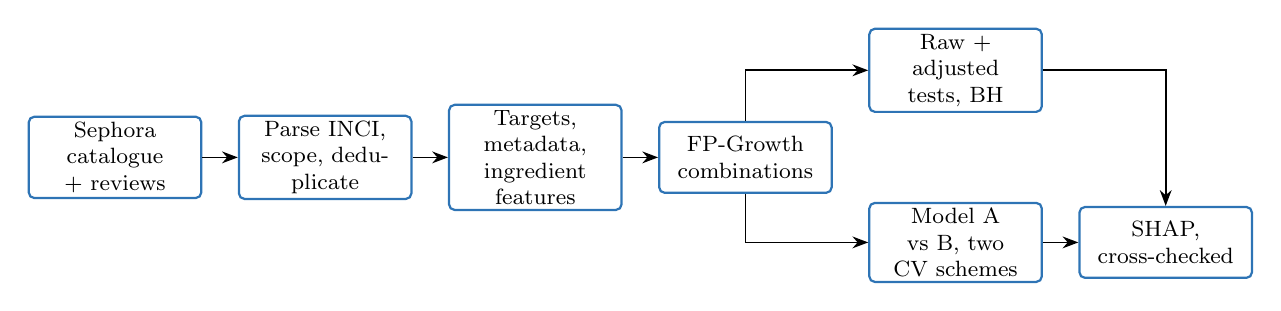
\begin{tikzpicture}[
  box/.style={draw=headblue, thick, rounded corners=2pt, align=center, font=\footnotesize, minimum height=0.9cm, text width=2.05cm, inner sep=2pt},
  arr/.style={-{Stealth[length=2mm]}, semithick}, node distance=0.4cm and 0.45cm]
\node[box] (raw) {Sephora catalogue\\+ reviews};
\node[box, right=of raw] (prep) {Parse INCI, scope, deduplicate};
\node[box, right=of prep] (feat) {Targets, metadata, ingredient features};
\node[box, right=of feat] (fp) {FP-Growth combinations};
\node[box, above right=0.1cm and 0.45cm of fp] (stats) {Raw + adjusted tests, BH};
\node[box, below right=0.1cm and 0.45cm of fp] (ml) {Model A vs B, two CV schemes};
\node[box, right=of ml] (shap) {SHAP, cross-checked};
\draw[arr] (raw) -- (prep); \draw[arr] (prep) -- (feat); \draw[arr] (feat) -- (fp);
\draw[arr] (fp) |- (stats); \draw[arr] (fp) |- (ml); \draw[arr] (ml) -- (shap);
\draw[arr] (stats.east) -| (shap.north);
\end{tikzpicture}
\caption{Analysis pipeline. All steps are deterministic and seeded; no language model is involved.}
\label{fig:pipeline}
\end{figure}

\subsection{Dataset, Scope and Deduplication}
We use the public Sephora product and review dataset~\cite{sephoradata}, whose catalogue lists \NCatalogue{} products with brand, category hierarchy, price, average rating, review count, ``loves'' count and the raw ingredient (INCI) text (Fig.~\ref{fig:pipeline}). Ingredient strings were parsed into ordered entities, keeping nested parentheses and colour-index groups intact, and labelled as primary ingredients or ``may contain'' shade lists; only primary ingredients are used, with spellings canonicalised (e.g.\ \emph{aqua/water/eau} becomes \emph{water}). We keep single-formula products with an ingredient list, excluding multi-component kits, gift sets, minis and tools, which leaves \NInScope{} products. A mini and its full-size version share one formula, and keeping both would place the same formula in training and test folds. We therefore merge products into families when they share a brand and either the same name after removing size words or an identical ingredient list, keeping the member with the most reviews. This yields \NAnalysed{} products.

\subsection{Success Indicators}
\emph{Rating} is the catalogue average, used only for products with at least 25 reviews (\NRating{} products). \emph{Popularity} is $\log(1+\text{loves})$ and \emph{engagement} is $\log(1+\text{reviews})$. \emph{Recommendation rate} is the share of reviewers recommending the product, from at least 25 votes; reviews exist for Skincare only, so it covers \NRecRate{} products. \emph{High performer} is a binary label for the top quartile of a composite that averages within-category percentile ranks of a shrunken rating, log loves and log reviews, so that the label does not simply encode the category. Rating and recommendation rate are nearly interchangeable (Spearman $\rho=0.94$), whereas rating and popularity are weakly negatively related ($\rho=-0.15$), so we model the indicators separately.

\subsection{Feature Sets and Combination Mining}
\emph{Baseline features (Model A)} are what a retailer knows without reading the label: brand and three category levels (one-hot, with brands of fewer than 10 products pooled); log price; value-price, on-sale, limited-edition, new, online-only, out-of-stock and exclusive flags; and variant count. Existing popularity (log loves and log reviews) enters only for rating and recommendation rate, where it is not circular.

\emph{Ingredient features (added in Model B)}, \NIngredientFeatures{} in total, are: presence of the 300 most frequent ingredients; list prominence $1-r/n$ of the 100 most frequent ($r$ the zero-based rank among $n$ ingredients), a coarse proxy for concentration; the number of ingredients; the share of ingredients in each of 37 functional groups (e.g.\ humectant, emollient, UV filter) from a curated ingredient--function table; and \NCombinations{} combination indicators. Combinations are frequent itemsets mined with FP-Growth~\cite{han2000fpgrowth} within each category: two or three ingredients with support of at least 5\% and lift of at least 1.5, at most 30 per category so that fragrance allergen clusters do not dominate. Mining does not use the targets, so it introduces no outcome leakage. Two combinations named in our project proposal, glycerin + sodium hyaluronate and glycerin + hyaluronic acid, are always tested as pre-specified hypotheses.

\subsection{Association Tests}
For every scope (all products, and each category with at least 300 products), target and binary feature present in and absent from at least 30 products each, we run two tests. \emph{Raw}: the Mann--Whitney $U$ test~\cite{mann1947} with Cliff's $\delta$~\cite{cliff1993} for continuous targets, a $\chi^2$ test with Cram\'er's $V$ for the high-performer label, and the Kruskal--Wallis test~\cite{kruskal1952} with $\varepsilon^2$ for functional-group shares binned into none, low and high. \emph{Adjusted}: we regress the standardised target on the feature with brand and subcategory fixed effects and log price, so each coefficient compares products of the same brand and subcategory at the same price. All coefficients are computed at once via the Frisch--Waugh--Lovell theorem~\cite{frisch1933,lovell1963}, which gives exact per-feature OLS estimates, standard errors and 95\% confidence intervals. Within each scope and target, raw and adjusted $p$-values are corrected separately with Benjamini--Hochberg~\cite{benjamini1995}; an association is \emph{robust} if raw and adjusted $q<0.05$ with the same sign.

\subsection{Predictive Modelling and Explainability}
For each target we train three model families on baseline features (Model A) and on baseline plus ingredient features (Model B), on identical folds: ridge or logistic regression with the penalty tuned by inner cross-validation, Random Forest~\cite{breiman2001rf} and LightGBM~\cite{ke2017lightgbm}; classifiers are class-balanced. Primary metrics are $R^2$ and ROC-AUC. \emph{Random} validation is 5-fold cross-validation repeated three times; \emph{unseen-brand} validation uses five folds that each hold out whole brands, where ingredient information should help most if it carries signal. Because fold scores share training data, we test the per-fold B minus A difference with the corrected resampled $t$-test of Nadeau and Bengio~\cite{nadeau2003}, which inflates the variance by $(1/k + n_{test}/n_{train})$. Models use scikit-learn~\cite{pedregosa2011sklearn}; tests use SciPy and statsmodels~\cite{seabold2010statsmodels}.

We fit LightGBM Model B on all products of a scope and compute SHAP values~\cite{lundberg2017shap} with TreeExplainer. Global importance is the mean absolute SHAP value, summed per feature family (metadata, ingredients, functional groups, combinations); top ingredient features count as \emph{confirmed} only if they are robust associations with the same direction. Three robustness checks use LightGBM with Benjamini--Hochberg correction within each check: \emph{ablation} adds each ingredient feature family to Model A on its own and also trains on ingredient features alone; \emph{other categories} repeats the comparison within Makeup, Hair and Fragrance; \emph{sensitivity} sets the review threshold to 10 or 50 and turns family deduplication off.

% ===================================================================== 4 RESULTS AND DISCUSSION
\section{Results and Discussion}

\subsection{Most Raw Associations Are Brand and Category Effects}
Across \NTests{} feature tests, \NSigRaw{} are significant before adjustment ($q<0.05$). Only \NSigAdj{} remain significant once brand, subcategory and price are held fixed, and \NRobust{} pass both tests with the same sign (Fig.~\ref{fig:attrition}). The attrition is strongest in Fragrance: dozens of raw associations per target, of which at most one survives. Table~\ref{tab:robust} and Fig.~\ref{fig:assoc} list the largest robust associations; most are modest, about 0.2 to 0.5 outcome standard deviations.

\begin{figure}[htbp]
\centering
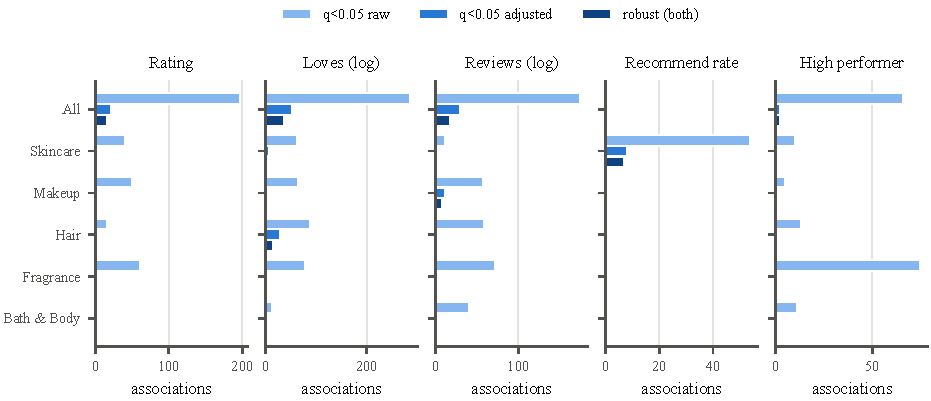
\includegraphics[width=0.92\textwidth]{fig_attrition.pdf}
\caption{Ingredient and combination associations with $q<0.05$ before adjustment (raw), after adjusting for brand, subcategory and price, and in both tests with the same sign (robust).}
\label{fig:attrition}
\end{figure}

The surviving associations are mostly not the actives products are marketed on. For rating, the strongest negative associations are vinylpyrrolidone film formers (VP/eicosene and VP/VA copolymers), typical of long-wear and styling formulas; positive ones include a ferment filtrate used as a preservative and the conditioning agent behentrimonium chloride. For popularity, the texture-giving silicone cyclopentasiloxane is the strongest positive association, while the anti-ageing peptide acetyl hexapeptide-8 is among the strongest negative ones. A plausible reading is that texture and wear, which shoppers experience directly, leave more trace in ratings and popularity than claimed actives do. These associations may still reflect product types finer than our subcategories, and we do not interpret them causally.

\begin{figure}[htbp]
\centering
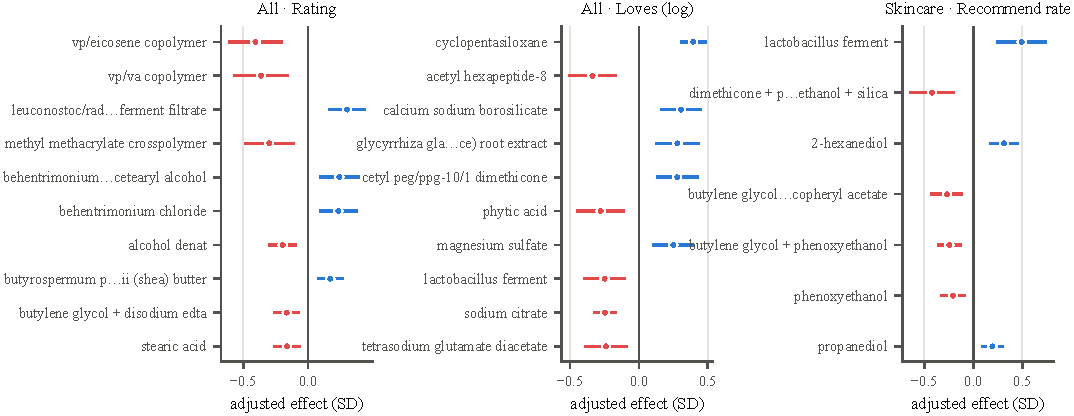
\includegraphics[width=0.95\textwidth]{fig_associations.pdf}
\caption{Largest robust associations: brand-, subcategory- and price-adjusted effect in outcome SD, with 95\% confidence intervals. Blue: positive; red: negative. Full names are in Table~\ref{tab:robust}.}
\label{fig:assoc}
\end{figure}

\begin{table}[htbp]
\centering
\footnotesize
\setlength{\tabcolsep}{3pt}
\begin{tabularx}{\linewidth}{|>{\raggedright\arraybackslash}X|l|r|r|r|c|r|}
\hline
\rowcolor{headfill} \textbf{Feature} & \textbf{Kind} & \textbf{$n$} & \textbf{Cliff's $\delta$} & \textbf{Adj.\ $\beta$} & \textbf{95\% CI} & \textbf{$q_{adj}$} \\
\hline
\multicolumn{7}{|l|}{\cellcolor{groupfill}\textbf{All, Rating}} \\
\hline
vp/eicosene copolymer & ingr. & 76 & $-0.471$ & $-0.407$ & [$-0.62$, $-0.19$] & 0.019 \\
\hline
vp/va copolymer & ingr. & 75 & $-0.291$ & $-0.364$ & [$-0.57$, $-0.15$] & 0.033 \\
\hline
leuconostoc/radish root ferment filtrate & ingr. & 211 & $+0.125$ & $+0.302$ & [$+0.16$, $+0.44$] & 0.005 \\
\hline
methyl methacrylate crosspolymer & ingr. & 91 & $-0.247$ & $-0.300$ & [$-0.49$, $-0.11$] & 0.048 \\
\hline
behentrimonium chloride + cetearyl alcohol & comb. & 163 & $+0.285$ & $+0.242$ & [$+0.09$, $+0.40$] & 0.048 \\
\hline
behentrimonium chloride & ingr. & 196 & $+0.258$ & $+0.234$ & [$+0.09$, $+0.38$] & 0.042 \\
\hline
\multicolumn{7}{|l|}{\cellcolor{groupfill}\textbf{All, Loves (log)}} \\
\hline
cyclopentasiloxane & ingr. & 301 & $+0.285$ & $+0.394$ & [$+0.30$, $+0.49$] & $<$0.001 \\
\hline
acetyl hexapeptide-8 & ingr. & 101 & $-0.222$ & $-0.337$ & [$-0.51$, $-0.16$] & 0.004 \\
\hline
calcium sodium borosilicate & ingr. & 116 & $+0.436$ & $+0.307$ & [$+0.16$, $+0.46$] & 0.003 \\
\hline
glycyrrhiza glabra (licorice) root extract & ingr. & 121 & $+0.277$ & $+0.280$ & [$+0.12$, $+0.44$] & 0.010 \\
\hline
cetyl peg/ppg-10/1 dimethicone & ingr. & 118 & $+0.467$ & $+0.279$ & [$+0.13$, $+0.43$] & 0.006 \\
\hline
phytic acid & ingr. & 88 & $-0.243$ & $-0.277$ & [$-0.45$, $-0.10$] & 0.022 \\
\hline
\multicolumn{7}{|l|}{\cellcolor{groupfill}\textbf{Skincare, Recommend rate}} \\
\hline
lactobacillus ferment & ingr. & 63 & $+0.207$ & $+0.493$ & [$+0.24$, $+0.75$] & 0.017 \\
\hline
dimethicone + phenoxyethanol + silica & comb. & 74 & $-0.189$ & $-0.424$ & [$-0.66$, $-0.19$] & 0.031 \\
\hline
2-hexanediol & ingr. & 290 & $+0.239$ & $+0.313$ & [$+0.17$, $+0.46$] & 0.009 \\
\hline
butylene glycol + phenoxyethanol + tocopheryl acetate & comb. & 175 & $-0.152$ & $-0.270$ & [$-0.43$, $-0.11$] & 0.049 \\
\hline
butylene glycol + phenoxyethanol & comb. & 455 & $-0.101$ & $-0.245$ & [$-0.37$, $-0.12$] & 0.015 \\
\hline
phenoxyethanol & ingr. & 813 & $-0.116$ & $-0.209$ & [$-0.33$, $-0.08$] & 0.049 \\
\hline
\end{tabularx}
\caption{Largest robust associations (raw and adjusted $q<0.05$, same sign).}
\label{tab:robust}
\end{table}


\subsection{Pre-specified Hypotheses}
Neither glycerin + sodium hyaluronate nor glycerin + hyaluronic acid is associated with rating (Table~\ref{tab:prespecified}). For popularity, glycerin + sodium hyaluronate shows a small negative adjusted association: among products of the same brand, subcategory and price, those containing the pair are slightly less loved, perhaps because the pair is too common in hydrating formulas to set a product apart. We treat this as a lead rather than a finding, because the raw test misses significance after correction and the association disappears without deduplication. The niacinamide + zinc combination from our project plan could not be tested, because zinc PCA is too rare in this catalogue.

\begin{table}[htbp]
\centering
\small
\begin{tabular}{|l|r|r|r|r|r|r|r|r|r|r|}
\hline
\rowcolor{headfill} \multicolumn{1}{|c|}{} & \multicolumn{5}{c|}{\textbf{All products}} & \multicolumn{5}{c|}{\textbf{Skincare}} \\
\hline
\rowcolor{headfill} \textbf{Target} & \textbf{$n$} & \textbf{Raw} & \textbf{$p$} & \textbf{Adj.\ $\beta$} & \textbf{$p_{adj}$} & \textbf{$n$} & \textbf{Raw} & \textbf{$p$} & \textbf{Adj.\ $\beta$} & \textbf{$p_{adj}$} \\
\hline
\multicolumn{11}{|l|}{\cellcolor{groupfill}\textbf{glycerin + sodium hyaluronate}} \\
\hline
Rating & 733 & $-0.003$ & 0.912 & $-0.006$ & 0.875 & 484 & $-0.024$ & 0.440 & $-0.074$ & 0.179 \\
\hline
Loves (log) & 884 & $-0.045$ & 0.033 & $-0.106$ & 0.001 & 589 & $-0.087$ & 0.003 & $-0.137$ & 0.002 \\
\hline
Reviews (log) & 884 & $+0.031$ & 0.143 & $-0.066$ & 0.056 & 589 & $-0.029$ & 0.317 & $-0.091$ & 0.054 \\
\hline
Recommend rate & 475 & $-0.005$ & 0.866 & $-0.045$ & 0.428 & 475 & $-0.005$ & 0.866 & $-0.045$ & 0.428 \\
\hline
High performer & 884 & $+0.013$ & 0.431 & $+0.022$ & 0.578 & 589 & $+0.002$ & 0.977 & $-0.021$ & 0.674 \\
\hline
\multicolumn{11}{|l|}{\cellcolor{groupfill}\textbf{glycerin + hyaluronic acid}} \\
\hline
Rating & 91 & $+0.045$ & 0.459 & $+0.054$ & 0.589 & 69 & $+0.055$ & 0.439 & $+0.065$ & 0.585 \\
\hline
Loves (log) & 112 & $+0.049$ & 0.377 & $-0.118$ & 0.134 & 87 & $+0.069$ & 0.279 & $-0.075$ & 0.430 \\
\hline
Reviews (log) & 112 & $+0.007$ & 0.895 & $-0.078$ & 0.351 & 87 & $-0.025$ & 0.689 & $-0.071$ & 0.481 \\
\hline
Recommend rate & 69 & $+0.099$ & 0.162 & $+0.096$ & 0.426 & 69 & $+0.099$ & 0.162 & $+0.096$ & 0.426 \\
\hline
High performer & 112 & $+0.091$ & 0.037 & $+0.195$ & 0.036 & 87 & $+0.148$ & 0.003 & $+0.336$ & 0.002 \\
\hline
\end{tabular}
\par\smallskip
\parbox{0.95\linewidth}{\footnotesize Raw: Cliff's $\delta$ (rate difference for high performer). Adj.\ $\beta$: brand-, subcategory- and price-adjusted difference in outcome SD. Unadjusted for multiple testing because the hypotheses were stated in advance. Recommendation rate exists for Skincare only.}
\caption{Pre-specified combinations from the project proposal.}
\label{tab:prespecified}
\end{table}


\subsection{Ingredient Features Add No Significant Predictive Value}
Model B is significantly better than Model A in \NBBetter{} of \NComparisons{} comparisons and significantly worse in \NABetter{} (Fig.~\ref{fig:models}, Table~\ref{tab:models}). For LightGBM, the model best suited to many sparse features, the largest mean gain is \MaxLGBMGain{} and no gain is significant under either validation scheme. The significant losses come from the linear models and the Random Forest, for technical reasons rather than because ingredients are harmful. A ridge or logistic model applies one penalty to all columns, and no single strength suits both the few dense metadata features and hundreds of sparse ingredient indicators. A Random Forest samples a fraction of features at each split, so hundreds of weak columns lower the chance that the strong brand and category features are available. LightGBM, which can ignore uninformative columns, neither gains nor loses significantly. This mirrors the finding of Aulya and Kusnawi~\cite{aulya2025} that seller reputation and price, not product content, drive predicted success.

\begin{figure}[htbp]
\centering
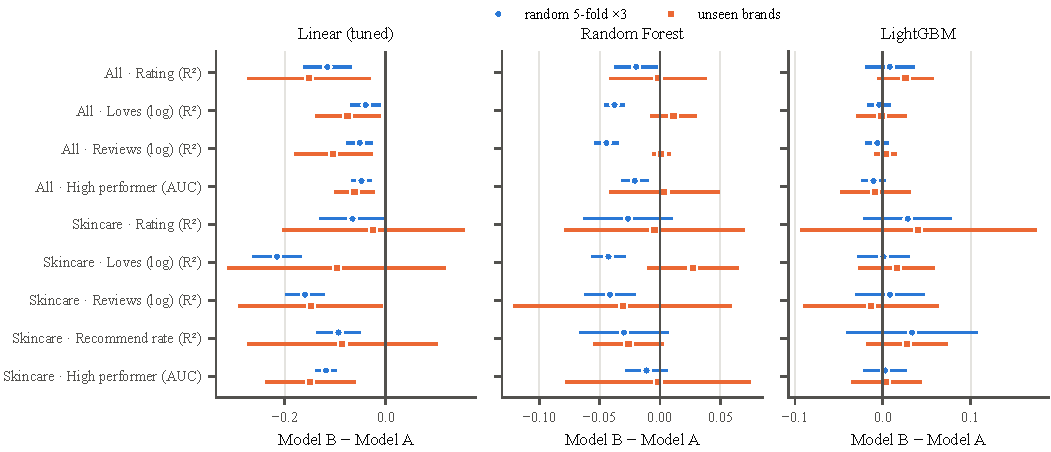
\includegraphics[width=0.9\textwidth]{fig_model_comparison.pdf}
\caption{Model B minus Model A on the primary metric ($R^2$, or ROC-AUC for high performer): mean over folds with 95\% intervals from the corrected resampled variance. Intervals crossing zero indicate no significant difference.}
\label{fig:models}
\end{figure}

\begin{table}[htbp]
\centering
\small
\begin{tabular}{|l|l|l|r|r|r|r|r|r|r|r|}
\hline
\rowcolor{headfill} \multicolumn{3}{|c|}{} & \multicolumn{4}{c|}{\textbf{Random 5-fold $\times$3}} & \multicolumn{4}{c|}{\textbf{Unseen brand}} \\
\hline
\rowcolor{headfill} \textbf{Scope} & \textbf{Target} & \textbf{Metric} & \textbf{A} & \textbf{B} & \textbf{$\Delta$} & \textbf{$p_{corr}$} & \textbf{A} & \textbf{B} & \textbf{$\Delta$} & \textbf{$p_{corr}$} \\
\hline
All & Rating & $R^2$ & 0.242 & 0.250 & $+0.008$ & 0.540 & 0.115 & 0.141 & $+0.026$ & 0.085 \\
\hline
All & Loves (log) & $R^2$ & 0.525 & 0.520 & $-0.004$ & 0.509 & 0.346 & 0.345 & $-0.001$ & 0.901 \\
\hline
All & Reviews (log) & $R^2$ & 0.438 & 0.432 & $-0.006$ & 0.339 & 0.276 & 0.280 & $+0.003$ & 0.505 \\
\hline
All & High performer & AUC & 0.801 & 0.790 & $-0.011$ & 0.125 & 0.745 & 0.736 & $-0.009$ & 0.582 \\
\hline
\hline
Skincare & Rating & $R^2$ & 0.176 & 0.204 & $+0.028$ & 0.243 & 0.025 & 0.065 & $+0.040$ & 0.451 \\
\hline
Skincare & Loves (log) & $R^2$ & 0.441 & 0.441 & $+0.001$ & 0.950 & 0.169 & 0.185 & $+0.016$ & 0.362 \\
\hline
Skincare & Reviews (log) & $R^2$ & 0.334 & 0.343 & $+0.008$ & 0.655 & 0.150 & 0.137 & $-0.013$ & 0.655 \\
\hline
Skincare & Recommend rate & $R^2$ & 0.199 & 0.233 & $+0.034$ & 0.348 & 0.124 & 0.151 & $+0.027$ & 0.176 \\
\hline
Skincare & High performer & AUC & 0.773 & 0.776 & $+0.003$ & 0.804 & 0.705 & 0.709 & $+0.004$ & 0.794 \\
\hline
\end{tabular}
\par\smallskip
\parbox{0.95\linewidth}{\footnotesize $p_{corr}$: Nadeau--Bengio corrected resampled $t$-test over folds (15 random, 5 unseen brand). Differences significant at 0.05: 0 of 18.}
\caption{Model A (metadata) vs Model B (+ingredient features), LightGBM.}
\label{tab:models}
\end{table}


\subsection{Attribution Is Not Added Value}
Although adding ingredients does not improve prediction, the ingredient-aware model attributes \MinIngredientShare{} to \MaxIngredientShare{}\% of its mean absolute SHAP value to ingredient-derived features (Fig.~\ref{fig:shapgap}). Ingredient features partly encode brand and category, because brands reuse bases and preservative systems across their ranges, and a tree ensemble given both can split on either. Read in isolation, the SHAP summary would suggest that ingredients drive success; the controlled comparison shows that they add nothing beyond the metadata. This is the dependence problem described by Aas et al.~\cite{aas2021} and Hooker et al.~\cite{hooker2021}, observed in real data.

Ingredients are not uninformative in themselves. A model given only ingredient features reaches $R^2=\OnlyRatingRTwo$ for rating, \OnlyLovesRTwo{} for popularity and \OnlyReviewsRTwo{} for review count, and a ROC-AUC of \OnlyHPAUC{} for the high-performer label (Table~\ref{tab:ablation}), against \ARatingRTwo, \ALovesRTwo, \AReviewsRTwo{} and \AHPAUC{} for metadata alone. Ingredients therefore carry real information about success, but less than metadata and, since adding them to metadata changes nothing, essentially the same information.

\begin{figure}[htbp]
\centering
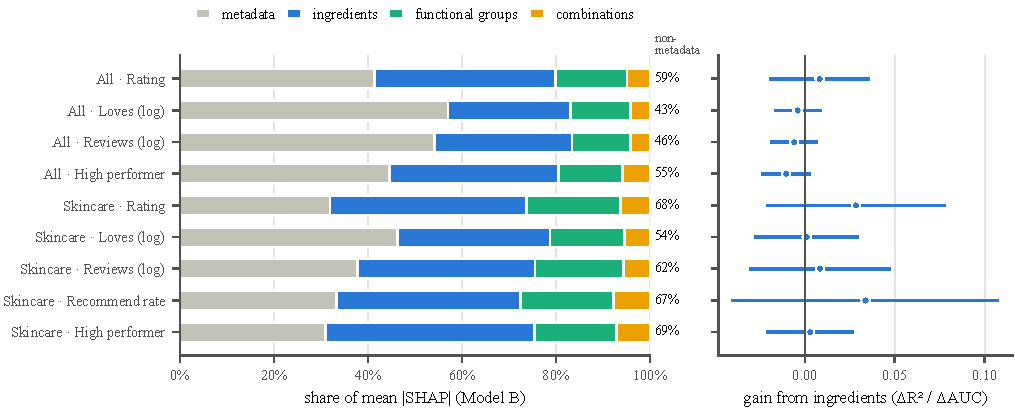
\includegraphics[width=0.9\textwidth]{fig_shap_gap.pdf}
\caption{Left: share of mean absolute SHAP value by feature family in Model B (LightGBM); the percentage is the non-metadata share. Right: the actual gain in $R^2$ or ROC-AUC from adding those features (random CV, 95\% corrected intervals).}
\label{fig:shapgap}
\end{figure}

\subsection{Robustness}
\emph{Ablation} (Table~\ref{tab:ablation}). Of \NAblationTests{} comparisons that add a single ingredient feature family to Model A, \NAblationNominal{} have a nominal $p<0.05$ and none survives correction (smallest $q=\MinAblationQ$). Individual ingredients and combinations lean positive, most clearly for Skincare rating and recommendation rate, while functional-group shares lean negative. \emph{Other categories} (Table~\ref{tab:categories}). Model B's largest gains appear in Fragrance, whose ingredient list is effectively its scent profile; \NCategoryNominal{} of \NCategoryTests{} comparisons have a nominal $p<0.05$ and none survives correction (smallest $q=\MinCategoryQ$). \emph{Sensitivity} (Table~\ref{tab:sensitivity}). With the review threshold at 10 or 50, or without family deduplication, no setting yields a significant gain: \NSensitivityNominal{} nominal and \NSensitivityFDR{} corrected out of \NSensitivityTests{} comparisons.

The null result for the full ingredient feature set is therefore robust to model choice, validation scheme, review threshold and deduplication. The point estimates nevertheless suggest where a better-powered study should look: individual ingredients in Skincare, and the ingredient list of fragrances.

\begin{table}[htbp]
\centering
\small
\begin{tabular}{|l|l|r|r|r|r|r|r|r|r|}
\hline
\rowcolor{headfill} \multicolumn{3}{|c|}{} & \multicolumn{2}{c|}{\textbf{+ ingredients}} & \multicolumn{2}{c|}{\textbf{+ functional}} & \multicolumn{2}{c|}{\textbf{+ combinations}} & \multicolumn{1}{c|}{\textbf{Ingr.\ only}} \\
\hline
\rowcolor{headfill} \textbf{Scope} & \textbf{Target} & \textbf{A} & \textbf{$\Delta$} & \textbf{$q$} & \textbf{$\Delta$} & \textbf{$q$} & \textbf{$\Delta$} & \textbf{$q$} & \textbf{Score} \\
\hline
All & Rating & 0.242 & $+0.011$ & 0.692 & $-0.003$ & 0.906 & $+0.011$ & 0.163 & 0.082 \\
\hline
All & Loves (log) & 0.525 & $+0.002$ & 0.906 & $-0.012$ & 0.129 & $+0.005$ & 0.623 & 0.193 \\
\hline
All & Reviews (log) & 0.438 & $-0.001$ & 0.906 & $-0.016$ & 0.129 & $+0.002$ & 0.732 & 0.107 \\
\hline
All & High performer & 0.801 & $-0.008$ & 0.598 & $-0.014$ & 0.163 & $+0.000$ & 0.906 & 0.640 \\
\hline
\hline
Skincare & Rating & 0.176 & $+0.062$ & 0.163 & $+0.002$ & 0.906 & $+0.041$ & 0.189 & 0.049 \\
\hline
Skincare & Loves (log) & 0.441 & $+0.019$ & 0.189 & $-0.022$ & 0.306 & $+0.007$ & 0.732 & 0.070 \\
\hline
Skincare & Reviews (log) & 0.334 & $+0.016$ & 0.659 & $-0.021$ & 0.318 & $-0.003$ & 0.906 & 0.040 \\
\hline
Skincare & Recommend rate & 0.199 & $+0.056$ & 0.272 & $+0.013$ & 0.844 & $+0.046$ & 0.163 & 0.034 \\
\hline
Skincare & High performer & 0.773 & $+0.010$ & 0.732 & $-0.025$ & 0.163 & $-0.004$ & 0.844 & 0.628 \\
\hline
\end{tabular}
\par\smallskip
\parbox{0.95\linewidth}{\footnotesize A: Model A score ($R^2$, or ROC-AUC for high performer). $\Delta$: gain over A from adding one feature family. $q$: Benjamini--Hochberg over all single-family variants. Ingr.\ only: a model with ingredient features and no metadata.}
\caption{Ablation of ingredient feature families (LightGBM, random CV).}
\label{tab:ablation}
\end{table}

\begin{table}[htbp]
\centering
\small
\begin{tabular}{|l|l|r|r|r|r|r|r|}
\hline
\rowcolor{headfill} \multicolumn{2}{|c|}{} & \multicolumn{3}{c|}{\textbf{Random}} & \multicolumn{3}{c|}{\textbf{Unseen brand}} \\
\hline
\rowcolor{headfill} \textbf{Scope} & \textbf{Target} & \textbf{$\Delta$} & \textbf{$p_{corr}$} & \textbf{$q$} & \textbf{$\Delta$} & \textbf{$p_{corr}$} & \textbf{$q$} \\
\hline
Makeup & Rating & $+0.009$ & 0.653 & 0.825 & $+0.062$ & 0.057 & 0.313 \\
\hline
Makeup & Loves (log) & $-0.002$ & 0.914 & 0.954 & $+0.019$ & 0.466 & 0.822 \\
\hline
Makeup & Reviews (log) & $-0.012$ & 0.614 & 0.822 & $+0.015$ & 0.295 & 0.770 \\
\hline
Makeup & High performer & $-0.008$ & 0.523 & 0.822 & $+0.018$ & 0.701 & 0.842 \\
\hline
\hline
Hair & Rating & $+0.058$ & 0.077 & 0.313 & $+0.070$ & 0.490 & 0.822 \\
\hline
Hair & Loves (log) & $+0.001$ & 0.957 & 0.957 & $+0.039$ & 0.549 & 0.822 \\
\hline
Hair & Reviews (log) & $+0.012$ & 0.617 & 0.822 & $+0.016$ & 0.831 & 0.949 \\
\hline
Hair & High performer & $-0.029$ & 0.078 & 0.313 & $-0.033$ & 0.545 & 0.822 \\
\hline
\hline
Fragrance & Rating & $+0.104$ & 0.047 & 0.313 & $+0.068$ & 0.566 & 0.822 \\
\hline
Fragrance & Loves (log) & $+0.005$ & 0.887 & 0.954 & $+0.120$ & 0.046 & 0.313 \\
\hline
Fragrance & Reviews (log) & $+0.030$ & 0.239 & 0.718 & $+0.059$ & 0.321 & 0.770 \\
\hline
Fragrance & High performer & $+0.033$ & 0.029 & 0.313 & $+0.042$ & 0.220 & 0.718 \\
\hline
\end{tabular}
\par\smallskip
\parbox{0.95\linewidth}{\footnotesize $q$: Benjamini--Hochberg over all rows and both splits of this table.}
\caption{Model B minus Model A within further categories (LightGBM).}
\label{tab:categories}
\end{table}

\begin{table}[htbp]
\centering
\small
\begin{tabular}{|l|l|r|r|r|r|r|r|}
\hline
\rowcolor{headfill} \multicolumn{2}{|c|}{} & \multicolumn{2}{c|}{\textbf{reviews $\geq$ 10 (5,547)}} & \multicolumn{2}{c|}{\textbf{reviews $\geq$ 50 (5,547)}} & \multicolumn{2}{c|}{\textbf{no deduplication (6,320)}} \\
\hline
\rowcolor{headfill} \textbf{Scope} & \textbf{Target} & \textbf{$\Delta$} & \textbf{$q$} & \textbf{$\Delta$} & \textbf{$q$} & \textbf{$\Delta$} & \textbf{$q$} \\
\hline
All & Rating & $-0.001$ & 0.921 & $+0.007$ & 0.838 & $+0.024$ & 0.561 \\
\hline
All & Loves (log) & $-0.004$ & 0.921 & $-0.004$ & 0.838 & $-0.010$ & 0.561 \\
\hline
All & Reviews (log) & $-0.004$ & 0.673 & $-0.004$ & 0.700 & $-0.006$ & 0.725 \\
\hline
All & High performer & $-0.012$ & 0.573 & $-0.012$ & 0.409 & $+0.003$ & 0.725 \\
\hline
\hline
Skincare & Rating & $+0.025$ & 0.573 & $+0.095$ & 0.409 & $+0.057$ & 0.561 \\
\hline
Skincare & Loves (log) & $-0.003$ & 0.921 & $-0.003$ & 0.904 & $-0.033$ & 0.561 \\
\hline
Skincare & Reviews (log) & $+0.010$ & 0.921 & $+0.010$ & 0.838 & $+0.012$ & 0.698 \\
\hline
Skincare & Recommend rate & $+0.038$ & 0.673 & $+0.047$ & 0.700 & $+0.040$ & 0.561 \\
\hline
Skincare & High performer & $-0.007$ & 0.921 & $-0.007$ & 0.838 & $+0.006$ & 0.725 \\
\hline
\end{tabular}
\par\smallskip
\parbox{0.95\linewidth}{\footnotesize $\Delta$: Model B minus Model A. $q$: Benjamini--Hochberg within each setting. Product counts in parentheses.}
\caption{Sensitivity of the Model A vs B comparison (LightGBM, 5-fold).}
\label{tab:sensitivity}
\end{table}


\subsection{Discussion}
\emph{What the null result means.} In this catalogue, how well a product is rated, loved or reviewed is explained largely by who makes it, what kind of product it is and what it costs. Ingredient lists carry information about success, but almost none that brand, category and price do not already carry. This does not show that ingredients are irrelevant to how a product performs on the skin: our outcomes are market outcomes, and our features record presence and order, not dose. It does show that an ingredient list, read from the label, is a weak and largely redundant signal of market success.

\emph{Why ingredients still look important.} Brands have formulation habits (house bases, preservative systems, signature fragrances), so an ingredient profile is partly a fingerprint of the brand and product type. A raw comparison picks up that fingerprint as an ``effect'', and a tree ensemble given both metadata and ingredients can split on either, so SHAP distributes credit between them; in the terms of Geirhos et al.~\cite{geirhos2020}, the ingredients act as a shortcut to brand. Attribution answers ``what did this model use?'', not ``what does this feature add?'' The gap between the two, \MinIngredientShare{} to \MaxIngredientShare{}\% of attribution with no significant gain, is in our view the most general lesson of the study.

\emph{Implications.} Claims that an ingredient drives ratings or sales, whether made by brands, retailers or ingredient-checker tools, should be tested against comparable products of the same brand and type, not against the market average. More generally, feature-importance results from observational data should be accompanied by an incremental test, such as a with/without comparison or held-out groups, before features are described as drivers~\cite{molnar2022}.

\subsection{Limitations}
The data are observational and come from a single retailer at a single point in time: success is also shaped by marketing, shelf placement and brand history, which we do not observe, and delisted products are absent (survivorship bias). Presence is not dose: list position is only a coarse proxy for concentration, and ingredients below 1\% may be listed in any order. Functional-group shares rely on a curated table that maps only part of all ingredient occurrences. Recommendation rate exists for Skincare only, and ratings cluster in a narrow, high range, which limits how much any model can explain. All findings are associations in this dataset; none is a causal, medical or safety claim.

% ===================================================================== 5 CONCLUSION
\section{Conclusion \& Future Scope}
We asked whether ingredient composition is associated with the market success of cosmetic products beyond brand, category and price. Most raw ingredient--success associations disappear once brand and subcategory are held fixed. Adding \NIngredientFeatures{} ingredient features to a metadata model yields no significant gain under random or unseen-brand validation, a result that holds across ablations, categories and data-construction choices. Ingredient features nonetheless receive a large share of SHAP attribution, because they largely re-encode brand and product type. Ingredient-based success claims, and feature-attribution claims in general, therefore need explicit control for confounders.

Concentration data, rather than list position, would allow ingredient doses to be tested. Within-brand reformulations of the same product, where the brand stays fixed and the formula changes, would offer a cleaner natural experiment. Catalogues from other retailers would show whether the weak signals we observe in Skincare and Fragrance generalise, and dependence-aware attribution methods~\cite{aas2021} could be compared with plain SHAP to quantify how much of the attribution gap they close.

% ===================================================================== 6 ACKNOWLEDGMENT
\section{Acknowledgment}
We thank Ms.\ Anshika Negi, Assistant Professor, Department of Information Technology, Bhagwan Parshuram Institute of Technology, for her guidance and supervision throughout this project. We are grateful to the creators of the publicly available Sephora product and review dataset~\cite{sephoradata}, and to the open-source communities behind scikit-learn, LightGBM, SHAP, SciPy, statsmodels, pandas and mlxtend, on which this work relies.

% ===================================================================== REFERENCES
% Same entries and order as references.tex ([1]-[15] = Table 1), set smaller and tighter.
% [16] is filled in as in the submitted PDF; references.tex still has a TODO there.
\begingroup\small
\begin{thebibliography}{99}
\setlength{\itemsep}{0pt}
\setlength{\parskip}{1pt}

\bibitem{chevalier2006}
J. A. Chevalier and D. Mayzlin, ``The Effect of Word of Mouth on Sales: Online Book Reviews,'' \emph{Journal of Marketing Research}, vol.~43, no.~3, pp.~345--354, 2006. \url{https://doi.org/10.1509/jmkr.43.3.345}

\bibitem{babic2016}
A. Babi\'{c} Rosario, F. Sotgiu, K. De Valck, and T. H. A. Bijmolt, ``The Effect of Electronic Word of Mouth on Sales: A Meta-Analytic Review of Platform, Product, and Metric Factors,'' \emph{Journal of Marketing Research}, vol.~53, no.~3, pp.~297--318, 2016. \url{https://doi.org/10.1509/jmr.14.0380}

\bibitem{moen2017}
{\O}. Moen, L. J. Havro, and E. Bjering, ``Online Consumers Reviews: Examining the Moderating Effects of Product Type and Product Popularity on the Review Impact on Sales,'' \emph{Cogent Business \& Management}, vol.~4, no.~1, p.~1368114, 2017. \url{https://doi.org/10.1080/23311975.2017.1368114}

\bibitem{aulya2025}
F. U. Aulya and K. Kusnawi, ``Evaluating Classification Models for Predicting Product Success in Indonesian E-Commerce,'' \emph{Jurnal Teknik Informatika (JUTIF)}, vol.~6, no.~4, pp.~2723--2739, 2025. \url{https://doi.org/10.52436/1.jutif.2025.6.4.5071}

\bibitem{sari2026}
Y. P. P. Sari, A. D. Hartanto, and I. N. Fajri, ``Skincare Product Recommendation System Using Hybrid Ensemble Learning,'' \emph{Journal of Applied Informatics and Computing}, vol.~10, no.~2, pp.~1587--1597, 2026. \url{https://doi.org/10.30871/jaic.v10i2.10461}

\bibitem{lee2024}
J. Lee, H. Yoon, S. Kim, C. Lee, J. Lee, and S. Yoo, ``Deep Learning-Based Skin Care Product Recommendation: A Focus on Cosmetic Ingredient Analysis and Facial Skin Conditions,'' \emph{Journal of Cosmetic Dermatology}, vol.~23, no.~6, pp.~2066--2077, 2024. \url{https://doi.org/10.1111/jocd.16218}

\bibitem{wang2025}
S. Wang, M. Nian, Y. Ma, X. Chen, X. Ji, C. Shi, X. Chen, and M. Fang, ``Machine Learning-Based Screening of Cosmetic Ingredients Identifies Vat Blue 6 as a Thyroid Hormone Receptor $\beta$ Disruptor,'' \emph{Environmental Science \& Technology}, vol.~59, no.~29, pp.~15005--15016, 2025. \url{https://doi.org/10.1021/acs.est.5c04327}

\bibitem{shim2024}
J. Shim, J. Woo, H. Yeo, S. Kang, B. Kwon, E. J. Lee, J. Oh, E. Jeong, J. Lim, and S. G. Park, ``The Clean Beauty Trend Among Millennial and Generation Z Consumers: Assessing the Safety, Ethicality, and Sustainability Attributes of Cosmetic Products,'' \emph{SAGE Open}, vol.~14, no.~2, 2024. \url{https://doi.org/10.1177/21582440241255430}

\bibitem{rizqia2026}
Y. N. Rizqia and A. Ichwani, ``Analisis Sentimen Ulasan Produk Skincare Sephora Menggunakan Algoritma BERT,'' \emph{Al-Kharaj: Jurnal Ekonomi, Keuangan \& Bisnis Syariah}, vol.~8, no.~9, pp.~4570--4581, 2026. \url{https://doi.org/10.47467/alkharaj.v8i9.13279}

\bibitem{lundberg2017shap}
S. M. Lundberg and S.-I. Lee, ``A Unified Approach to Interpreting Model Predictions,'' in \emph{Advances in Neural Information Processing Systems 30 (NeurIPS 2017)}, 2017. \url{https://arxiv.org/abs/1705.07874}

\bibitem{kumar2020}
I. E. Kumar, S. Venkatasubramanian, C. Scheidegger, and S. Friedler, ``Problems with Shapley-Value-Based Explanations as Feature Importance Measures,'' in \emph{Proceedings of the 37th International Conference on Machine Learning}, PMLR vol.~119, pp.~5491--5500, 2020. \url{https://proceedings.mlr.press/v119/kumar20e.html}

\bibitem{aas2021}
K. Aas, M. Jullum, and A. L{\o}land, ``Explaining Individual Predictions When Features Are Dependent: More Accurate Approximations to Shapley Values,'' \emph{Artificial Intelligence}, vol.~298, p.~103502, 2021. \url{https://doi.org/10.1016/j.artint.2021.103502}

\bibitem{hooker2021}
G. Hooker, L. Mentch, and S. Zhou, ``Unrestricted Permutation Forces Extrapolation: Variable Importance Requires at Least One More Model, or There Is No Free Variable Importance,'' \emph{Statistics and Computing}, vol.~31, no.~6, p.~82, 2021. \url{https://doi.org/10.1007/s11222-021-10057-z}

\bibitem{molnar2022}
C. Molnar, G. K\"{o}nig, J. Herbinger, T. Freiesleben, S. Dandl, C. A. Scholbeck, G. Casalicchio, M. Grosse-Wentrup, and B. Bischl, ``General Pitfalls of Model-Agnostic Interpretation Methods for Machine Learning Models,'' in \emph{xxAI: Beyond Explainable AI}, Lecture Notes in Computer Science, vol.~13200, pp.~39--68, 2022. \url{https://doi.org/10.1007/978-3-031-04083-2_4}

\bibitem{geirhos2020}
R. Geirhos, J.-H. Jacobsen, C. Michaelis, R. Zemel, W. Brendel, M. Bethge, and F. A. Wichmann, ``Shortcut Learning in Deep Neural Networks,'' \emph{Nature Machine Intelligence}, vol.~2, no.~11, pp.~665--673, 2020. \url{https://doi.org/10.1038/s42256-020-00257-z}

\bibitem{sephoradata}
N. Inky, ``Sephora Products and Skincare Reviews,'' Kaggle, 2023. \url{https://www.kaggle.com/datasets/nadyinky/sephora-products-and-skincare-reviews}

\bibitem{benjamini1995}
Y. Benjamini and Y. Hochberg, ``Controlling the False Discovery Rate: A Practical and Powerful Approach to Multiple Testing,'' \emph{Journal of the Royal Statistical Society: Series B (Methodological)}, vol.~57, no.~1, pp.~289--300, 1995. \url{https://doi.org/10.1111/j.2517-6161.1995.tb02031.x}

\bibitem{nadeau2003}
C. Nadeau and Y. Bengio, ``Inference for the Generalization Error,'' \emph{Machine Learning}, vol.~52, no.~3, pp.~239--281, 2003. \url{https://doi.org/10.1023/A:1024068626366}

\bibitem{han2000fpgrowth}
J. Han, J. Pei, and Y. Yin, ``Mining Frequent Patterns without Candidate Generation,'' in \emph{Proceedings of the 2000 ACM SIGMOD International Conference on Management of Data}, pp.~1--12, 2000. \url{https://doi.org/10.1145/342009.335372}

\bibitem{ke2017lightgbm}
G. Ke, Q. Meng, T. Finley, T. Wang, W. Chen, W. Ma, Q. Ye, and T.-Y. Liu, ``LightGBM: A Highly Efficient Gradient Boosting Decision Tree,'' in \emph{Advances in Neural Information Processing Systems 30 (NeurIPS 2017)}, 2017.

\bibitem{breiman2001rf}
L. Breiman, ``Random Forests,'' \emph{Machine Learning}, vol.~45, no.~1, pp.~5--32, 2001. \url{https://doi.org/10.1023/A:1010933404324}

\bibitem{cliff1993}
N. Cliff, ``Dominance Statistics: Ordinal Analyses to Answer Ordinal Questions,'' \emph{Psychological Bulletin}, vol.~114, no.~3, pp.~494--509, 1993. \url{https://doi.org/10.1037/0033-2909.114.3.494}

\bibitem{mann1947}
H. B. Mann and D. R. Whitney, ``On a Test of Whether One of Two Random Variables Is Stochastically Larger than the Other,'' \emph{The Annals of Mathematical Statistics}, vol.~18, no.~1, pp.~50--60, 1947. \url{https://doi.org/10.1214/aoms/1177730491}

\bibitem{kruskal1952}
W. H. Kruskal and W. A. Wallis, ``Use of Ranks in One-Criterion Variance Analysis,'' \emph{Journal of the American Statistical Association}, vol.~47, no.~260, pp.~583--621, 1952. \url{https://doi.org/10.1080/01621459.1952.10483441}

\bibitem{frisch1933}
R. Frisch and F. V. Waugh, ``Partial Time Regressions as Compared with Individual Trends,'' \emph{Econometrica}, vol.~1, no.~4, pp.~387--401, 1933. \url{https://doi.org/10.2307/1907330}

\bibitem{lovell1963}
M. C. Lovell, ``Seasonal Adjustment of Economic Time Series and Multiple Regression Analysis,'' \emph{Journal of the American Statistical Association}, vol.~58, no.~304, pp.~993--1010, 1963. \url{https://doi.org/10.1080/01621459.1963.10480682}

\bibitem{pedregosa2011sklearn}
F. Pedregosa \emph{et al.}, ``Scikit-learn: Machine Learning in Python,'' \emph{Journal of Machine Learning Research}, vol.~12, pp.~2825--2830, 2011. \url{https://jmlr.org/papers/v12/pedregosa11a.html}

\bibitem{seabold2010statsmodels}
S. Seabold and J. Perktold, ``Statsmodels: Econometric and Statistical Modeling with Python,'' in \emph{Proceedings of the 9th Python in Science Conference}, pp.~92--96, 2010. \url{https://doi.org/10.25080/Majora-92bf1922-011}

\end{thebibliography}
\endgroup

\end{document}
